

\tikzset{every picture/.style={line width=0.75pt}} %set default line width to 0.75pt        

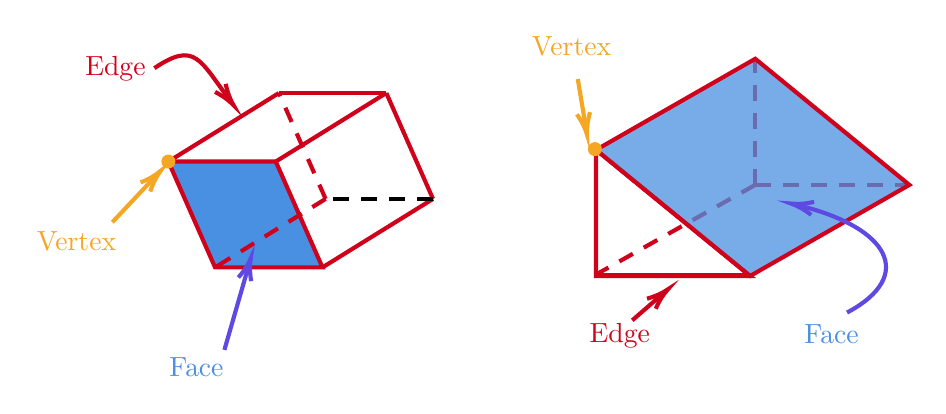
\begin{tikzpicture}[x=0.75pt,y=0.75pt,yscale=-1,xscale=1, scale= 0.75]
%uncomment if require: \path (0,288); %set diagram left start at 0, and has height of 288

%Shape: Rectangle [id:dp053370527561274805] 
\draw  [color={rgb, 255:red, 208; green, 2; blue, 27 }  ,draw opacity=1 ][fill={rgb, 255:red, 74; green, 144; blue, 226 }  ,fill opacity=1 ][line width=1.5]  (130,96) -- (199,96) -- (229,164) -- (160,164) -- cycle ;
%Straight Lines [id:da7233344038492684] 
\draw [color={rgb, 255:red, 208; green, 2; blue, 27 }  ,draw opacity=1 ][line width=1.5]    (199,96) -- (270,52) ;


%Straight Lines [id:da8870385695360932] 
\draw [color={rgb, 255:red, 208; green, 2; blue, 27 }  ,draw opacity=1 ][line width=1.5]    (130,96) -- (201,52) ;


%Straight Lines [id:da6880167264201218] 
\draw [color={rgb, 255:red, 208; green, 2; blue, 27 }  ,draw opacity=1 ][line width=1.5]    (229,164) -- (300,120) ;


%Straight Lines [id:da8629284451428976] 
\draw [color={rgb, 255:red, 208; green, 2; blue, 27 }  ,draw opacity=1 ][line width=1.5]    (300,120) -- (270,52) ;


%Straight Lines [id:da5801797655392487] 
\draw [color={rgb, 255:red, 208; green, 2; blue, 27 }  ,draw opacity=1 ][line width=1.5]    (270,52) -- (201,52) ;


%Straight Lines [id:da33437733704095596] 
\draw [color={rgb, 255:red, 208; green, 2; blue, 27 }  ,draw opacity=1 ][line width=1.5]  [dash pattern={on 5.63pt off 4.5pt}]  (231,120) -- (201,52) ;


%Straight Lines [id:da7324938230911522] 
\draw [line width=1.5]  [dash pattern={on 5.63pt off 4.5pt}]  (300,120) -- (231,120) ;


%Straight Lines [id:da04595951918657737] 
\draw [color={rgb, 255:red, 208; green, 2; blue, 27 }  ,draw opacity=1 ][line width=1.5]  [dash pattern={on 5.63pt off 4.5pt}]  (231,120) -- (160,164) ;


%Shape: Right Triangle [id:dp15828119672901897] 
\draw  [color={rgb, 255:red, 208; green, 2; blue, 27 }  ,draw opacity=1 ][line width=1.5]  (404.75,88.5) -- (503.75,169.5) -- (404.75,169.5) -- cycle ;
%Straight Lines [id:da18371357143649392] 
\draw [color={rgb, 255:red, 208; green, 2; blue, 27 }  ,draw opacity=1 ][line width=1.5]  [dash pattern={on 5.63pt off 4.5pt}]  (507,111) -- (507,30) ;


%Straight Lines [id:da5323303129683379] 
\draw [color={rgb, 255:red, 208; green, 2; blue, 27 }  ,draw opacity=1 ][line width=1.5]  [dash pattern={on 5.63pt off 4.5pt}]  (507,111) -- (606,111) ;


%Straight Lines [id:da1934412072495324] 
\draw [color={rgb, 255:red, 208; green, 2; blue, 27 }  ,draw opacity=1 ][line width=1.5]  [dash pattern={on 5.63pt off 4.5pt}]  (404,169) -- (507,111) ;


%Curve Lines [id:da9915257466456324] 
\draw [color={rgb, 255:red, 208; green, 2; blue, 27 }  ,draw opacity=1 ][line width=1.5]    (121,36) .. controls (147.33,18.45) and (149.88,30.37) .. (170.39,57.86) ;
\draw [shift={(172,60)}, rotate = 232.82] [color={rgb, 255:red, 208; green, 2; blue, 27 }  ,draw opacity=1 ][line width=1.5]    (14.21,-4.28) .. controls (9.04,-1.82) and (4.3,-0.39) .. (0,0) .. controls (4.3,0.39) and (9.04,1.82) .. (14.21,4.28)   ;

%Shape: Circle [id:dp6348766282723517] 
\draw  [draw opacity=0][fill={rgb, 255:red, 245; green, 166; blue, 35 }  ,fill opacity=1 ] (125.5,96) .. controls (125.5,93.51) and (127.51,91.5) .. (130,91.5) .. controls (132.49,91.5) and (134.5,93.51) .. (134.5,96) .. controls (134.5,98.49) and (132.49,100.5) .. (130,100.5) .. controls (127.51,100.5) and (125.5,98.49) .. (125.5,96) -- cycle ;
%Straight Lines [id:da9603817642462407] 
\draw [color={rgb, 255:red, 245; green, 166; blue, 35 }  ,draw opacity=1 ][line width=1.5]    (94,135) -- (122.95,104.19) ;
\draw [shift={(125,102)}, rotate = 493.21] [color={rgb, 255:red, 245; green, 166; blue, 35 }  ,draw opacity=1 ][line width=1.5]    (14.21,-4.28) .. controls (9.04,-1.82) and (4.3,-0.39) .. (0,0) .. controls (4.3,0.39) and (9.04,1.82) .. (14.21,4.28)   ;

%Straight Lines [id:da6450171763852104] 
\draw [color={rgb, 255:red, 94; green, 74; blue, 226 }  ,draw opacity=1 ][line width=1.5]    (166,217) -- (182.17,160.88) ;
\draw [shift={(183,158)}, rotate = 466.07] [color={rgb, 255:red, 94; green, 74; blue, 226 }  ,draw opacity=1 ][line width=1.5]    (14.21,-4.28) .. controls (9.04,-1.82) and (4.3,-0.39) .. (0,0) .. controls (4.3,0.39) and (9.04,1.82) .. (14.21,4.28)   ;

%Shape: Polygon [id:ds14971897219625419] 
\draw  [color={rgb, 255:red, 208; green, 2; blue, 27 }  ,draw opacity=1 ][fill={rgb, 255:red, 74; green, 144; blue, 226 }  ,fill opacity=0.75 ][line width=1.5]  (507,30) -- (606,111) -- (503.75,169.5) -- (404.75,88.5) -- cycle ;
%Straight Lines [id:da1871099492645416] 
\draw [color={rgb, 255:red, 208; green, 2; blue, 27 }  ,draw opacity=1 ][line width=1.5]    (503,169) -- (404,169) ;


%Straight Lines [id:da5598317572787015] 
\draw [color={rgb, 255:red, 208; green, 2; blue, 27 }  ,draw opacity=1 ][line width=1.5]    (428,198) -- (448.74,179.97) ;
\draw [shift={(451,178)}, rotate = 498.99] [color={rgb, 255:red, 208; green, 2; blue, 27 }  ,draw opacity=1 ][line width=1.5]    (14.21,-4.28) .. controls (9.04,-1.82) and (4.3,-0.39) .. (0,0) .. controls (4.3,0.39) and (9.04,1.82) .. (14.21,4.28)   ;

%Shape: Circle [id:dp5936650276871587] 
\draw  [draw opacity=0][fill={rgb, 255:red, 245; green, 166; blue, 35 }  ,fill opacity=1 ] (399.5,88) .. controls (399.5,85.51) and (401.51,83.5) .. (404,83.5) .. controls (406.49,83.5) and (408.5,85.51) .. (408.5,88) .. controls (408.5,90.49) and (406.49,92.5) .. (404,92.5) .. controls (401.51,92.5) and (399.5,90.49) .. (399.5,88) -- cycle ;
%Straight Lines [id:da46178057371883363] 
\draw [color={rgb, 255:red, 245; green, 166; blue, 35 }  ,draw opacity=1 ][line width=1.5]    (393,43) -- (398.51,76.04) ;
\draw [shift={(399,79)}, rotate = 260.54] [color={rgb, 255:red, 245; green, 166; blue, 35 }  ,draw opacity=1 ][line width=1.5]    (14.21,-4.28) .. controls (9.04,-1.82) and (4.3,-0.39) .. (0,0) .. controls (4.3,0.39) and (9.04,1.82) .. (14.21,4.28)   ;

%Curve Lines [id:da39173533566192775] 
\draw [color={rgb, 255:red, 94; green, 74; blue, 226 }  ,draw opacity=1 ][line width=1.5]    (566,193) .. controls (610.33,169.36) and (593.53,137.96) .. (532.8,123.64) ;
\draw [shift={(530,123)}, rotate = 372.53] [color={rgb, 255:red, 94; green, 74; blue, 226 }  ,draw opacity=1 ][line width=1.5]    (14.21,-4.28) .. controls (9.04,-1.82) and (4.3,-0.39) .. (0,0) .. controls (4.3,0.39) and (9.04,1.82) .. (14.21,4.28)   ;


% Text Node
\draw (96,36) node  [align=left] {\textcolor[rgb]{0.82,0.01,0.11}{Edge}};
% Text Node
\draw (71,147) node  [align=left] {\textcolor[rgb]{0.96,0.65,0.14}{Vertex}};
% Text Node
\draw (148,228) node [color={rgb, 255:red, 74; green, 144; blue, 226 }  ,opacity=1 ] [align=left] {\textcolor[rgb]{0.29,0.56,0.89}{Face}};
% Text Node
\draw (420,208) node  [align=left] {\textcolor[rgb]{0.82,0.01,0.11}{Edge}};
% Text Node
\draw (556,207) node [color={rgb, 255:red, 74; green, 144; blue, 226 }  ,opacity=1 ] [align=left] {\textcolor[rgb]{0.29,0.56,0.89}{Face}};
% Text Node
\draw (389,22) node  [align=left] {\textcolor[rgb]{0.96,0.65,0.14}{Vertex}};
% % Text Node
% \draw (198,268) node   {$( a)$};
% % Text Node
% \draw (485,268) node   {$( b)$};


\end{tikzpicture}